\scanpage{20}
\LMpagefigure{\figure{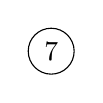
\begin{tikzpicture}
\node[draw,circle,inner sep=3pt] {\mspage{7}};
\end{tikzpicture}}}{7}

\diagram{\begin{tikzcd}[ampersand replacement=\&,column sep=1.6em,row sep=2.8em,column sep=9pt,row sep=14pt,execute at begin picture={\fontsize{10}{12}\selectfont}]
\&\&
\begin{gathered}
\widetilde\rho=(\rho_0,2)=(\rho,2)\\
\widetilde\sigma=(\sigma_0,3)=(\sigma,3)
\end{gathered}
\arrow[d, bend right=20]
\&
\begin{gathered}
\deleted{\unsure{\Pi_{0,3}^{D}}}\\[-2pt]
\inserted{\text{\uline{\unsure{identifié à}}}}\\[-2pt]
\inserted{\unsure{S\mathcal T_{11}\times_{\Pi_{0,3}^{D}}\mathbb Z/12\mathbb Z}}
\end{gathered}
\arrow[d]
\&
\begin{gathered}
\rho_0=(\rho,\dot 2)\\[-2pt]
\unsure{\Pi_{0,3}}\\[-2pt]
\sigma_0=(\sigma,\dot 3)=(\sigma,-1)
\end{gathered}
\arrow[d]
\&\\
\unsure{0|1}\arrow[r,dash]\&
\mathbb Z\arrow[r,dash,"1\unsure{-|\mapsto}\overline\omega=\omega^2"]\arrow[dd,equal]\&
S\mathcal T_{11}\arrow[r,Rightarrow]\arrow[dd,"\substack{\widetilde\rho\mapsto\deleted{\unsure{4}}2\\\widetilde\sigma\mapsto3}"']
\arrow[ddr,phantom,"\text{Cart}"]\&
\mathcal T_{11}\arrow[r,Rightarrow]\arrow[dr,leftrightarrow]\arrow[dd,"\substack{\rho_0\mapsto\dot 2\\\sigma_0\mapsto\dot 3}"']
\&\Pi_{0,3}^{\prime D}\arrow[dr,"\text{can}"]\arrow[dd,"\substack{\rho\mapsto2\\\sigma\mapsto3}"{pos=.25,xshift=2pt}]
\arrow[dl,phantom,"\text{cart}" description]\&\\
\&\&\&{}\&
|[xshift=-3em]|\mathbb D'_3\arrow[r,"\text{cart}"{pos=.75}]\arrow[dd]
\&\mathbb D_3\arrow[dd,"\text{can}"]\\
1\arrow[r,dash]\&\mathbb Z\arrow[r,"12"]\&\mathbb Z\arrow[r,"\text{can}"]\&
\mathbb Z/12\mathbb Z\arrow[r,"\text{can}"]\arrow[dr,"\text{can}"']
\&\mathbb Z/6\mathbb Z\arrow[dr,"\text{can}"]
\arrow[d,phantom,"\text{\uline{Cart}}"'{pos=.25,xshift=-3.5em,yshift=4pt}]
\arrow[dr,phantom,"\text{\uline{cart}}"{description,xshift=-1.5em,yshift=-.5em}]\&\\
\&\&\&\&\mathbb Z/4\mathbb Z\arrow[r,leftrightarrow,"\text{can}"']\&\mathbb Z/2\mathbb Z
\end{tikzcd}}

\margin{\unsure{pour} $\mathcal T_{11}$ \unsure{identifié à}
$\Pi_{0,3}^{D}\times_{\mathbb Z/2\mathbb Z}\mathbb Z/4\mathbb Z$}

\unsure{A-t-on} \unsure{bien}\quad
$\bigm|\quad S\mathcal T_{11}\simeq S\Pi_{0,3}^{D}$ ??

il semblerait plutôt, pourtant
\[
\deleted{\unsure{\mathcal T_{11}}}\quad
PM_{11}\simeq
\left(\underbrace{T^*U_{0,3}}_{\substack{\text{fibré}\\\text{\uline{tangent}}}},\mathfrak S_3\right)
\]
\inserted{(et \uline{non} $\unsure{PU_{0,3}}$ !!)}

\[
\text{donc}\quad \mathcal T_{11}\simeq\pi_1(T^*U_{0,3},\mathfrak S_3)\ \ldots
\]
\margin{19}

\scanpage{21}
% Trois longs traits obliques au crayon, terminés chacun en crochet, traversent tout le feuillet : rature d'ensemble.
% Les ratures à l'encre (ligne « Op. ext. … », « compatible avec l'op. ext. », E corrigé en F, 1 et π_1 de la dernière suite) restent marquées à l'intérieur.
\deleted{
\[
\pi\qquad l_1\ \cdots\ l_n
\]

\diagram{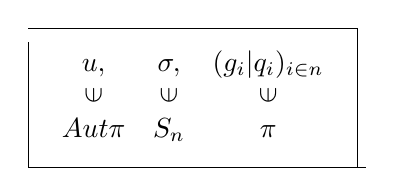
\begin{tikzpicture}
\node[inner sep=7pt] (p) {$\begin{array}{ccc}
u,&\sigma,&(\unsure{g_i|q_i})_{i\in n}\\
\rotatebox{90}{$\in$}&\rotatebox{90}{$\in$}&\rotatebox{90}{$\in$}\\
\operatorname{Aut}\pi&\mathfrak S_n&\pi
\end{array}$};
\draw (p.north west) -- (p.north east) -- (p.south east);
\draw ([yshift=-5pt]p.north west) -- (p.south west) -- ([xshift=3pt]p.south east);
\end{tikzpicture}}
\diagram{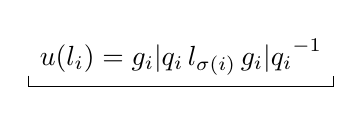
\begin{tikzpicture}
\node[inner sep=4pt] (u) {$u(l_i)=\unsure{g_i|q_i}\,l_{\sigma(i)}\,\unsure{g_i|q_i}^{-1}$};
\draw ([yshift=4pt]u.south west) -- (u.south west) -- (u.south east) -- ([yshift=4pt]u.south east);
\end{tikzpicture}}

\diagram{\begin{tikzcd}[ampersand replacement=\&,column sep=1.5em]
1\arrow[r,dash]\&\pi_1(\operatorname{Aut}(X)\arrow[r]\&\mathbb Z^n\arrow[r]\&S\mathcal T\arrow[r]\&\mathcal T\arrow[r,dash]\&\mathfrak S_n\arrow[r,dash]\&1
\end{tikzcd}}

\diagram{\begin{tikzpicture}
\node[inner sep=9pt] (b) {\begin{tikzcd}[ampersand replacement=\&,column sep=3em,row sep=2.5em]
\pi\arrow[r,hook]\&\widetilde E\arrow[r]\arrow[d,leftrightarrow]\&\mathfrak S_n\\
\unsure{\mathfrak Z\pi|\mathfrak z\pi}\arrow[u]\arrow[r]\&\mathbb Z^n\&{}
\end{tikzcd}};
\draw (b.north west) -- (b.north east) -- ([yshift=2pt]b.east) -- ([xshift=-6pt]b.east)
 -- ([xshift=-12pt,yshift=5pt]b.south east) -- ([xshift=0.7cm,yshift=5pt]b.south)
 -- ([xshift=0.6cm,yshift=-6pt]b.south) -- ([yshift=-6pt]b.south west) -- (b.north west);
\end{tikzpicture}}

\diagram{\begin{tikzcd}[ampersand replacement=\&,column sep=2.3em,row sep=1.8em]
\&\&1\&\&\\
1\arrow[r]\&\underbrace{S\operatorname{Aut}^{+}(X)}\arrow[r]\arrow[d,"\simeq"]\&
\operatorname{Aut}^{+}(X)\arrow[u]\arrow[r,dash]\&\operatorname{Aut}^{+}(\partial X)\arrow[r,dash]\&1\\
\&\uline{S\mathcal T}\&\operatorname{Aut}^{+}_{!}(\widetilde X)\arrow[u]\&\uline{\mathfrak S_n\cdot\mathbb T^n}\arrow[u,"\simeq"]\&\\
\&\&\pi\arrow[u]\&\&\\
\&\&1\arrow[u]\&\&
\end{tikzcd}}

\diagram{\begin{tikzcd}[ampersand replacement=\&,column sep=1.6em]
1\arrow[r,dash]\&\underbrace{\pi_1\operatorname{Aut}^{+}(X)}_{0\ \text{ou}\ \mathbb Z}\arrow[r,Rightarrow]\&\mathbb Z^n\arrow[r,dash]\&S\mathcal T\arrow[r,dash]\&\mathcal T\arrow[r,dash]\&\mathfrak S_n\arrow[r,dash]\&1
\end{tikzcd}}

\diagram{\begin{tikzpicture}
\node[inner sep=6pt] (e) {\begin{tikzcd}[ampersand replacement=\&,column sep=2em,row sep=1.8em]
1\arrow[r,dash]\&S\mathcal T\arrow[r,dash]\&E\arrow[r]\arrow[d,equal]\&\mathfrak S_n\arrow[r,dash]\&1\\
\&\mathbb Z^n\arrow[u]\&\widetilde E/\pi\&\&{}
\end{tikzcd}};
\draw ([xshift=5pt]e.north west) -- ([xshift=-7pt]e.north east)
 .. controls ([xshift=12pt]e.north east) and ([xshift=12pt,yshift=-1cm]e.north east) .. ([xshift=-4pt,yshift=-1.1cm]e.north east)
 -- ([xshift=-0.5cm,yshift=-1.1cm]e.north)
 .. controls ([xshift=-0.8cm,yshift=-1.2cm]e.north) and ([xshift=-0.8cm,yshift=-0.3cm]e.south) .. ([xshift=-1.5cm]e.south)
 .. controls (e.south west) and ([xshift=-8pt]e.west) .. ([yshift=-4pt]e.north west);
\end{tikzpicture}}

\diagram{\begin{tikzcd}[ampersand replacement=\&,column sep=2.4em,row sep=2em]
1\arrow[r,dash]\&\unsure{\widetilde F|\widehat F}\arrow[r,dash]\arrow[d]\&\widetilde A\arrow[r,dash]\arrow[d]\&\widetilde G\arrow[d]\&\\
1\arrow[r,dash]\&\substack{\deleted{\unsure{E}}\inserted{F}\\\text{discret}}\arrow[r]\&A\arrow[r]\&G\arrow[dr]\&
\bigl(=\mathfrak S_n\unsure{\ast|\cdot}\mathbb T^n\bigr)\\
\&\&\&\&1
\end{tikzcd}}

\deleted{\unsure{Op.} ext. de $\pi_0$ sur $F$}

\diagram{\begin{tikzcd}[ampersand replacement=\&,column sep=3.8em,row sep=2.3em]
\pi_1(G)=\pi_1\arrow[r]\arrow[dr,bend right=20,"\substack{\text{\unsure{compatible}}\\\text{avec }\pi_0}"']\&F\arrow[d,phantom,"\cup" description]\\
\&\unsure{\mathfrak Z(F)|\mathfrak z(F)}
\end{tikzcd}}
\inserted{\unsure{central}}

$\pi_0(G)=\pi_0$ opère \unsure{extérieurement} sur $F$
\quad donc opère sur $\unsure{\mathfrak Z(F)|\mathfrak z(F)}$

\diagram{$\begin{array}{cc}
\pi_0&\pi_1\\
\multicolumn{2}{c}{\text{op.}}
\end{array}$}
\deleted{\unsure{compatible} avec l'op. ext.}

\diagram{\begin{tikzcd}[ampersand replacement=\&,column sep=2.4em,row sep=1.7em]
1\arrow[r,dash]\&F\arrow[r]\&E\arrow[r]\arrow[d,equal]\&\pi_0\arrow[r,dash]\&1\\
\&\&\pi_0(\widetilde A)\&\&{}
\end{tikzcd}}
\figure{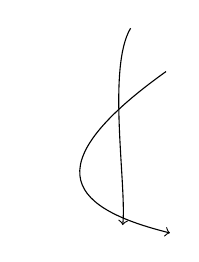
\begin{tikzpicture}[x=1cm,y=1cm]
\draw[->] (0.3,2.5) .. controls (0.0,2.0) and (0.25,0.5) .. (0.2,0);
\draw[->] (0.75,1.95) .. controls (-1.0,0.7) and (-0.4,0.2) .. (0.8,-0.1);
\end{tikzpicture}}

\diagram{\begin{tikzcd}[ampersand replacement=\&,column sep=1.6em]
1\arrow[r,dash]\&\pi_1(A)\arrow[r,dash]\&\pi_1\arrow[r]\&\unsure{F}\arrow[r]\&\underbrace{\pi_0(A)}\arrow[r]\&\substack{\unsure{\pi_0|\pi_\infty}\\ /}\arrow[r,dash]\&1
\end{tikzcd}}

\diagram{\begin{tikzcd}[ampersand replacement=\&,column sep=1.7em,row sep=1.5em,nodes in empty cells]
\deleted{\unsure{1}}\arrow[r,dash]\&\deleted{\unsure{\pi_1}}\arrow[r,dash]\&F\arrow[r,dash]\&\pi_0(\widetilde A)\arrow[r]\arrow[d,equal]\&\pi_0\arrow[r]\&1\\
\&\&\&E\&\&{}
\end{tikzcd}}
}
\margin{20}

\scanpage{22}
% blank
\margin{21}

\scanpage{23}
A)\quad \uline{Lemme}\quad
$S$ schéma \deleted{\unsure{satisfaisant|strictement}}
régulier intègre tel que $\operatorname{Pic}(S)=0$,
car. du point générique $\ne2$ Alors \deleted{$\unsure{H^1}$}
\[
H^1(U_{0,3},\mathfrak S_3;\mathbb G_m]\simeq\mathbb Z/6\mathbb Z
\]
(\deleted{\unsure{résiduelle}}\inserted{\unsure{pt gén.|si gén.}} est $2$, on trouve $\mathbb Z/3\mathbb Z$)

\margin{\uline{\unsure{Dém}}\quad on utilise suite exacte
\diagram{\begin{tikzcd}[ampersand replacement=\&,column sep=1.3em,row sep=2em]
0\arrow[r]\&H^1(\mathfrak S_3,H^0(U_{0,3},\mathbb G_m)\arrow[r]\&H^1(\text{mixte})\arrow[dll]\&{}\\
H^0\bigl(\mathfrak S_3,\underbrace{H^1(U_{0,3};\mathbb G_m)}_{0}\bigr)\&\&\&{}
\end{tikzcd}}
et
\diagram{\begin{tikzcd}[ampersand replacement=\&,column sep=1.3em]
0\arrow[r]\&H^0(S,\mathbb G_m)\arrow[r]\&H^0(U_{0,3},\mathbb G_m)\arrow[r]\&\unsure{h_1(V(J))|h^1(V(J))}\arrow[r]\&0
\end{tikzcd}}}

\unsure{Je} dis que si \inserted{le schéma}
$\deleted{\unsure{U_{0,3}}}\inserted{\Sigma_J}$ est défini comme $\mathbb P(V_J)$, \unsure{i.e.}
\diagram{\begin{tikzcd}[ampersand replacement=\&,column sep=2.8em]
0\arrow[r,dash]\&V_J\arrow[r]\&\mathcal O^J\arrow[r]\&\mathcal O\arrow[r,dash]\&0
\end{tikzcd}}
alors le fibré \unsure{principal}
\[
P\Sigma_J=\check V(\mathcal O_{\Sigma_J}(1))^{*}
\]
est un générateur du
$H^1(\deleted{\unsure{U_{0,3}}}\inserted{\Sigma_J^*},
\deleted{\unsure{\mathfrak S_3}}\inserted{\mathfrak S_J};\mathbb G_m)$.

Je vais d'abord \unsure{trouver} une trivialisation de
\[
\uline{\mathcal O}(1)^{\otimes6}=\mathcal O(6)\simeq
\unsure{\mathcal T^{\otimes3}(\omega)|\mathcal J^{\otimes3}(\omega)},
\]
\deleted{donc} \inserted{en fait} une section de $\mathcal O(6)$
\inserted{sur $\overline\Sigma$ \unsure{tout entier}}
(qui \deleted{\unsure{ne s'annule que}}
\inserted{\unsure{est}, \unsure{inversible}} sur $\Sigma^*$.
On \deleted{\unsure{prenant}} a
\[
\Gamma(\Sigma_J,\mathcal O(6))\simeq\operatorname{Sym}^{6}V_J
\]
et on prendra
\[
\begin{gathered}
\unsure{\varphi|\Delta}\in\Gamma(\Sigma_J,\mathcal O(6)),\qquad
\unsure{\varphi|\Delta}
=\deleted{\unsure{\sum_{i\in J}}}
-\prod_{\substack{i,j\in J\\i\ne j}}(e_i-e_j)\\
=\prod_{i\in J}\underbrace{(e_j-e_h)}_{J=\{i,j,h\}}^{2}.
\end{gathered}
\]
Ainsi, sur $\deleted{\unsure{U_J}}\inserted{\Sigma_J^{*}}$, le groupe \unsure{structural|structurel}
\deleted{\unsure{de}}
$\mathbb G_m$ de $P\Sigma_J^{*}$ est réduit \unsure{à|:} $\mu_6$.

\uline{NB}\quad Sauf erreur, on a
\[
\deleted{\unsure{\operatorname{Sym}}}\quad
\operatorname{Sym}^{*}(V_J)^{\mathfrak S_3}\simeq
\mathcal O\bigl(\unsure{\gamma_2|\varphi_2},\unsure{\gamma_3|\varphi_3}\bigr)
/(2\gamma_3^2-\gamma_2^3)
\]
\[
\left\{\begin{aligned}
\gamma_2&=\sum_{i\in J}(e_j-e_h)^2\\
\gamma_3&=\prod_{i\in J}(e_j\unsure{-|+}e_h-2e_i)
\end{aligned}\right.
\qquad\text{et}\quad\Delta=\gamma_2^3
\]
\margin{22}

\scanpage{24}
% not manuscript: tract imprimé « Parler Femmes à propos de “PLURIELLES” », avec une longue rature diagonale.
\margin{23}

\scanpage{25}
\Needspace{14\baselineskip}
B)

\deleted{\unsure{Si} $2$ \unsure{inversible}, on \unsure{aura} \unsure{donc}}
\[
\deleted{\operatorname{Sym}^{*}(\unsure{V_J|W_J})^{\mathfrak S_{\unsure{J|3}}}\simeq\mathcal O[}
\]
\deleted{\unsure{Remarque}}

Comme $\gamma_2$ s'annule en \deleted{\unsure{les}} $P_\omega$,
$\gamma_3$ en les $Q_i$, il s'ensuit qu'il n'y a pas de section invariante
d'un $\mathcal O(n)^*$ \deleted{\unsure{pour}} sur
$\Sigma_J^{*}$ \deleted{\unsure{en degré} $<$}
pour $n\le6$, donc que l'ordre de
$\operatorname{cl}(\mathcal O(1))$ dans
$H^1(\Sigma_J,\mathfrak S_J;\mathbb G_m)$ est bien $6$,
ce qui \unsure{prouve} que $\mathcal O(1)$ est un générateur du
$\unsure{H^1}$ mixte.
\margin{24}
\scanpage{26}
% not manuscript: feuillet dactylographié « Sciences de l’homme », « Energie », « Mécanique et industries de transformation », « Recherches sur les milieux tropicaux et sub-tropicaux » ; pagination imprimée « - 4 - ».
\margin{25}

\scanpage{27}
% Étiquette imprimée, oblique et à l'envers sur le feuillet.
\begin{flushleft}
MR LE PROFESSEUR GROTHENDIECK ALEX.\\
MATHEMATIQUES\hfill 5
\end{flushleft}

\diagram{\begin{tikzcd}[ampersand replacement=\&,column sep=huge]
\mathbb D'_3 \arrow[r] \& \mathbb D_3
\end{tikzcd}}

\margin{\figure{\begin{tikzpicture}[x=1cm,y=1cm]
\draw (0,0) .. controls (.1,.14) and (.25,.13) .. (.48,.03);
\end{tikzpicture}}}

\diagram{\begin{tikzcd}[ampersand replacement=\&,column sep=large,row sep=large]
PM_{11}(2^{\sim})\overset{?}{\simeq}PU_{0,3}
  \arrow[r,very thick] \arrow[d,leftrightarrow]
\& PM_{11}(2)\simeq TU_{0,3} \arrow[d]\\
U_{0,3}\simeq M_{11}(\unsure{\widetilde{2}^{\sim}|2^{\sim}})
  \arrow[r,very thick]
\& \begin{gathered}(U_{0,3},\{1,\omega\})\\[-2pt]{}\simeq M_{11}(\unsure{2})\end{gathered}
\arrow[ul,phantom,"\mathrm{cart}" description]
\end{tikzcd}}

\[
\deleted{\unsure{x}\longrightarrow\unsure{x^2\wedge\omega_0}}
\]
\[
\unsure{H^1}(TU_{03},\mathbb D_3;\mu_2)
\]

\diagram{\begin{tikzcd}[ampersand replacement=\&,column sep=small,row sep=large]
M_{11}(2^{\sim}) \arrow[rr]
  \arrow[dr,"{\deleted{\unsure{\mathcal D/\Pi_{0,3}|\mathbb Z/2\,\Pi_{0,3}}}}"']
\& \& M_{11}(2)\unsure{-|'} \arrow[dl] \arrow[d,leftrightarrow] \& \phantom{M}\\
\& M_{11} \arrow[d] \& M_{11}(2)' \arrow[dl] \& \\
\phantom{M}\arrow[rrruu,dashed,no head,shorten <=-10pt,shorten >=-10pt]
\& M'_{11} \& \&
\end{tikzcd}}

\diagram{\begin{tikzcd}[ampersand replacement=\&,column sep=small,row sep=large]
U_{03} \arrow[rr,"{\{1,\omega\}}"] \arrow[dr,"{\mathbb D'_3}"']
\& \& (U_{0,3},\{1,\omega\}) \arrow[dl,"{\mathbb D_3}"'] \arrow[d,"{\unsure{\mathrm{gerbe}}}"] \& \phantom{U}\\
\& (U_{0,3},\mathbb D'_3) \arrow[d,"{\unsure{\mathrm{gerbe}}}"']
\& (U_{03}) \arrow[dl,"{\mathbb D_3}"] \& \\
\phantom{U}\arrow[rrruu,dashed,no head,shorten <=-12pt,shorten >=-12pt]
\& (U_{0,3},\mathbb D_3) \& \&
\end{tikzcd}}

\diagram{\begin{tikzcd}[ampersand replacement=\&,column sep=small,row sep=large]
\begin{gathered}(\mathcal D,\Pi_{03})\\[-2pt]{}\simeq\mathcal D/\Pi_{03}\end{gathered}
 \arrow[rr,very thick,"{\mathrm{gal}}","{\{1,\omega\}}"']
 \arrow[dr,"{\begin{gathered}\mathrm{gal}\\\mathbb D'_3\end{gathered}}"']
\& \& (\mathcal D,\Pi_{03}\times\{1,\omega\})
 \arrow[dl,"{\begin{gathered}\mathrm{gal}\\\mathbb D_3\ \deleted{\unsure{\{1,\omega\}}}\end{gathered}}"']
 \arrow[d,"{\unsure{2\text{-}\uline{\mathrm{gerbe}}}}"] \& \phantom{D}\\
\& (\mathcal D,\unsure{\mathrm{Sl}(2,\mathbb Z)})
 \arrow[d,"{\unsure{2\text{-}\mathrm{gerbe}}}"']
\& (\mathcal D,\Pi_{03}) \arrow[dl,"{\begin{gathered}\mathrm{gal}\\\mathbb D_3\end{gathered}}"] \& \\
\phantom{D}\arrow[rrruu,dashed,no head,shorten <=-12pt,shorten >=-12pt]
\& (\mathcal D,\unsure{\mathrm{Sl}(2,\mathbb Z)}') \& \&
\end{tikzcd}}

\margin{26}

\scanpage{28}
% not manuscript: avis dactylographié, à l’envers, de soutenance d’une thèse de doctorat de 3ème cycle, « Algèbres de Rees », YOON Suk-Im, Montpellier, le 26 février 1982 ; soutenance prévue le 4 MARS 1982 à 15h.
\margin{27}

\scanpage{29}

\deleted{\diagram{\begin{tikzcd}[ampersand replacement=\&,column sep=small,row sep=large]
\& \& {}\arrow[r,"{\unsure{''|1}}"]
\& \mathrm{Sl}(2,\mathbb Z)\arrow[r]\arrow[d]
\& \Pi_{0,3}^{D}\arrow[d] \& \\
\& \unsure{\widetilde\varepsilon|\widetilde E}\arrow[rr]
  \arrow[ddl]\arrow[dr,dashed]
\& \& \mathbb D_3\mathop{\times}\limits_{\mathbb Z/2\mathbb Z}
       \mathbb Z/\unsure{12}\mathbb Z
       \simeq\mathbb D'_3\mathop{\times}\limits_{\mathbb Z/\unsure{2}\mathbb Z}
       \mathbb Z/6\mathbb Z
       \arrow[r]\arrow[dd,very thick]\arrow[d,dashed]
\& \mathbb D_3\mathop{\times}\limits_{\mathbb Z/2\mathbb Z}
       \mathbb Z/6\mathbb Z=\unsure{\varepsilon|E}
       \arrow[dd]\arrow[dr] \& \\
\& \& \mathbb Z\arrow[r,no head]\arrow[ddl,dashed,leftrightarrow,very thick]
\& \mathbb Z/12\mathbb Z\arrow[rr,dashed,"{\mathrm{can}}"]
       \arrow[dd,dashed,"{\mathrm{can}}"'{pos=.2}]
\& \& \mathbb Z/6\mathbb Z\arrow[ddl,"{\mathrm{can}}"]\\
\unsure{\widetilde{\mathbb D}_3^{*}|\widetilde{\mathbb D}'_3}
 \arrow[rrr,very thick]\arrow[dr]
\& \& \& \mathbb D'_3\arrow[r,very thick]\arrow[d,very thick]
\& \mathbb D_3\arrow[d,"{\mathrm{can}}"] \& \\
\& \mathbb Z\arrow[rr] \& \& \mathbb Z/4\mathbb Z\arrow[r,"{\mathrm{can}}"]
\& \mathbb Z/2\mathbb Z \&
\end{tikzcd}}}

\figure{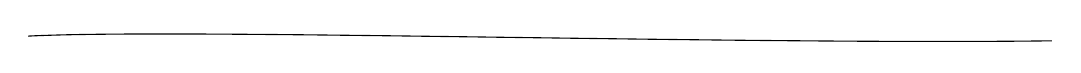
\begin{tikzpicture}[x=1cm,y=1cm]
\draw (0,.06) .. controls (2,.16) and (9,-.05) .. (13,0);
\end{tikzpicture}}

\diagram{\begin{tikzcd}[ampersand replacement=\&,column sep=small,row sep=large]
\unsure{\mathbb Z_{(\omega/2)}}\arrow[r]\arrow[d,very thick]
\& \widetilde\Pi_{0,3}^{\unsure{\circ}}
   \deleted{\unsure{\widetilde\Pi_{0,3}}}\arrow[rr,very thick]\arrow[d]
\& \& \Pi_{0,3}\arrow[d,leftrightarrow,bend left=12]
\& \& \& \\
\mathbb Z_{(\omega)}\arrow[r,very thick]\arrow[d,equal]
\& \widetilde\Pi_{0,3}^{\unsure{'}}\arrow[rr]\arrow[d,very thick]
\& \& \Pi'_{0,3}=\Pi_{0,3}\times\{1,\omega\}
   \arrow[rr]\arrow[d,bend right=12]
\& \& \Pi_{03}\arrow[d,bend right=18] \& \\
\mathbb Z\arrow[r,very thick]\arrow[d,equal]
\& \widetilde{\mathrm{Sl}}(2,\mathbb Z)=\widetilde\Pi_{0,3}^{D}
   \arrow[rr]\arrow[d]
\& \& \mathrm{Sl}(2,\mathbb Z)\arrow[rr]\arrow[d,very thick]\arrow[ddr]
\& \& \Pi_{0,3}^{D}\arrow[d]\arrow[ddr] \& \\
\mathbb Z\arrow[r]\arrow[dd,equal]
\& \widetilde{\mathbb D}_3\arrow[rr]\arrow[dd]
\& \& \begin{gathered}\mathbb D'''_3\\\margin{3}\end{gathered}\arrow[rr,"2"]\arrow[dr,"3"']\arrow[dd,"3"']
\& \& \begin{gathered}\mathbb D''_3\\\margin{\unsure{12|10}}\end{gathered}\arrow[dr,"3"]\arrow[dd,"3"'{pos=.72}] \& \\
\& \& \& \& \mathbb D'_3\arrow[rr,"2"{pos=.75}]\arrow[dd,"3"{pos=.77}]
\& \& \mathbb D_3\arrow[dd,"3"]\\
\mathbb Z\arrow[r,"12"]
\& \mathbb Z\arrow[rr]
\& \& \mathbb Z/12\mathbb Z\arrow[rr,leftrightarrow,"2"]\arrow[dr,"3"']
\& \& \mathbb Z/6\mathbb Z\arrow[dr,"3"] \& \\
\& \& \& \& \mathbb Z/4\mathbb Z\arrow[rr,"2"] \& \& \mathbb Z/2\mathbb Z
\end{tikzcd}}
\margin{\unsure{fond|bon}}

\diagram{\begin{tikzcd}[ampersand replacement=\&,column sep=large,row sep=large]
1\arrow[r,no head]
\& \mathbb Z\arrow[r,no head]\arrow[d,very thick,"{\begin{gathered}4\\\unsure{4}\end{gathered}}"]
\& \widetilde\Pi_{0,3}^{D}\arrow[r,no head]\arrow[d,no head]
\& \Pi_{0,3}^{D}\arrow[r]\arrow[d,no head]
\& 1\\
1\arrow[r,no head]
\& \mathbb Z\arrow[r,no head]
\& \widetilde\Pi_{0,3}^{D}(4)\arrow[r]
\& \Pi_{0,3}^{D}\arrow[r,very thick]
\& 1
\end{tikzcd}}

\figure{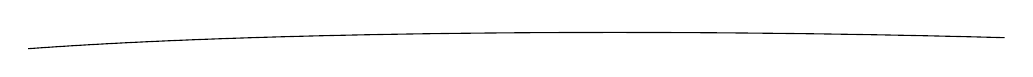
\begin{tikzpicture}[x=1cm,y=1cm]
\draw (0,0) .. controls (3,.22) and (8,.26) .. (12.4,.14);
\end{tikzpicture}}

\diagram{\begin{tikzcd}[ampersand replacement=\&,column sep=large,row sep=large]
\& \& \widetilde\Pi_{0,3}^{D}
\& \Pi_{0,3}^{D}\arrow[r,no head] \& 1\\
1\arrow[r]
\& \overset{\omega}{\mathbb Z}\arrow[r]
\& \widetilde\Pi_{0,3}^{D}(4)\arrow[r]
\& \Pi_{0,3}^{D}\times\mathbb Z/4\mathbb Z\arrow[u]\arrow[r,no head]
\& 1\\
1\arrow[r,no head]
\& \mathbb Z\arrow[r]
\& ?\arrow[r]
\& \unsure{\mathrm{Sl}(2,\mathbb Z)}\arrow[u]\arrow[r,no head]
\& 1
\end{tikzcd}}

\margin{28}

\scanpage{30}
% Secteur supérieur : un long trait courbe au crayon, terminé en crochet, descend de « par les e_i-e_j » vers le bas à gauche ;
% il traverse les trois premières lignes, la suite Z — Π̃_03 — Π_03 → 1 et la formule V(ω) ≃ V, barrées ici en bloc.
\deleted{
$V_J\deleted{\unsure{\simeq}}\inserted{=\unsure{\Gamma(X,\uline{\mathcal O}(1))}}
\deleted{e_i-e_j}$ \unsure{engendré} par les $e_i-e_j$

\deleted{$\unsure{\Pi(e_i-e_j)|P(e_i-e_j)}$}
\unsure{comment} ces \unsure{sections} \unsure{sont} elles
\unsure{permutées} entre elles
}

\figure{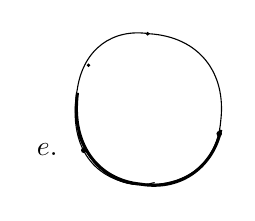
\begin{tikzpicture}[x=1cm,y=1cm]
\draw (0,.95) .. controls (.64,.91) and (.98,.45) .. (.91,-.15)
 .. controls (.86,-.78) and (.36,-1.04) .. (-.25,-.95)
 .. controls (-.83,-.83) and (-1.02,-.33) .. (-.91,.26)
 .. controls (-.83,.76) and (-.46,1.02) .. (0,.95);
\draw[line width=1.1pt] (-.91,.2) .. controls (-1,-.48) and (-.63,-.91) .. (-.11,-.96)
 .. controls (.43,-1.05) and (.82,-.71) .. (.91,-.27);
\draw (-.9,-.33) .. controls (-.72,-.82) and (-.31,-1.05) .. (.07,-.94);
\fill (-.02,.95) circle (.025);
\fill (-.77,.55) circle (.024);
\fill (-.83,-.53) circle (.035);
\fill (.89,-.32) circle (.035);
\node[left] at (-1.04,-.52) {$e.$};
\end{tikzpicture}}

\[
\deleted{e_i-e_j\qquad\unsure{\mathcal O(6)|\mathcal O(1)}}
\qquad e_i-e_j=
\]
\[
\unsure{\xi_i}.
\]

\diagram{\begin{tikzcd}[ampersand replacement=\&,column sep=small,row sep=small]
\unsure{\uline{\mathcal O}_x(1)|\uline{\mathcal O}_a(1)}\arrow[d,phantom,"{\unsure{\in}}"{description,rotate=90}]
 \& {}\ni\xi_{ij}(x)\\
\lambda \& \lambda^6=\displaystyle\prod_{i,j}\xi_{ij}(x)
\end{tikzcd}}

\deleted{\diagram{\begin{tikzcd}[ampersand replacement=\&,column sep=large]
\mathbb Z\arrow[r,no head]
\& \widetilde\Pi_{\unsure{03}}\arrow[r]
\& \Pi_{03}^{\unsure{\sharp|\ast}}\arrow[r,very thick]
\& 1
\end{tikzcd}}}

\[
(e_i-e_j)(\uline{\unsure{Q_n|Q_k}})
\qquad\deleted{\unsure{e_i-e_j}}
\]

\[
\deleted{\mathbf V(\omega)\overset{!!}{\simeq}\mathbf V}
\qquad \varphi\in V
\qquad e_i-e_j(\deleted{\unsure{Q_k}}\,
\]
\[
e_i-e_j\bmod L_{Q_k}
\]

\diagram{\(\begin{array}{ccc}
\frac12 & \frac12 & 1\\
-\frac12 & -\frac12 & -1
\end{array}\)}
\[
\left(\frac12\right)^4\qquad\sqrt[3]{\frac12}
\]

% Secteur inférieur, écrit à l'envers par rapport au secteur précédent.
\deleted{
On a vu qu'une orientation d'une \deleted{\unsure{surface}}\inserted{\unsure{carte}}
\inserted{\unsure{cellulaire|cellulation}} combinatoire $A$
\unsure{donne} lieu \unsure{à|:} deux \unsure{opérateurs|opérations}
$\vec\rho_s,\vec\rho_f$ sur $\vec A$, \unsure{satisfaisant}
\[
\vec\rho_s^{-1}\vec\rho_f=\sigma
\]

Si on prend l'orientation inverse, \unsure{quels|quelles} sont les
\unsure{opérateurs|opérations} \unsure{correspondants|correspondantes}
$\vec\rho'_s,\vec\rho'_f$ ?
Si $\vec a\in\vec A$ \unsure{provient} de $a\in A^L_+$,
il \unsure{provient} de $\sigma_na\in A^L_-$, et on a
\[
\rho_s(\sigma_na)
 =\sigma_n
   (\underbrace{\sigma_n\rho_s\sigma_n}
     _{\sigma_n\varepsilon=\rho_s^{-1}}a)
 =\sigma_n(\rho_s^{-1}a)\,-
\]
\unsure{donc} la classe dans $\vec A\simeq A^L/\sigma_n$
est celle de $\rho_s^{-1}a$,
i.e. $\vec\rho_s^{-1}\vec a$.
\deleted{\unsure{E}}t on a donc
\[
\deleted{\rho_f(\sigma_na)
 =\sigma_n
  (\underbrace{\sigma_n\rho_f\sigma_n}
   _{\sigma_n\varepsilon\sigma}a)}
\]
\[
\vec\rho'_s=\vec\rho_s^{-1}
\]
d'où
\[
\vec\rho'_f=\vec\rho'_s\sigma
 =\vec\rho_s^{-1}\sigma
 =\sigma\vec\rho_f^{-1}\sigma
 =\mathrm{int}(\sigma)\vec\rho_f^{-1}
\]
(Ce n'est pas tellement \unsure{plaisant}.)
}

\margin{
% Notes perpendiculaires dans la marge droite du secteur inférieur redressé.
\[
\unsure{\widetilde Q_m|\widetilde R_m}
 -\unsure{\widetilde Q_j|\widetilde R_j}
\]
\[
\deleted{\unsure{\xi}}\quad\unsure{\gamma_h\ i\gamma_h}
\]
\[
e_j-e_i\quad -(e_i-e_h)
\]
}

\margin{29}

\scanpage{31}

\deleted{\diagram{\begin{tikzcd}[ampersand replacement=\&,column sep=large,row sep=large,nodes in empty cells]
1\arrow[r,hook]
\& \mathbb Z\arrow[r,no head]
\& \widetilde\Pi\arrow[r]
\& \Pi\arrow[r,no head]\arrow[d]
\& 1\\
\& \& \& \deleted{\unsure{D''_3}} \&
\end{tikzcd}}}

\diagram{\begin{tikzcd}[ampersand replacement=\&,column sep=small,row sep=large]
\& \& \Pi_0\arrow[rr,equal]\arrow[dr]
\& \& \Pi_0\unsure{.}\arrow[dr] \& \& \\
\mathbb Z\arrow[r]\arrow[d,equal]
\& \widetilde\Pi\arrow[rr]\arrow[d]
\& \& \Pi'\arrow[rr]\arrow[d]\arrow[ddr]
\& \& \Pi\arrow[d]\arrow[ddr] \& \\
\mathbb Z\arrow[r]\arrow[dd,equal]
\& \widetilde D_{\unsure{3|0}}\arrow[rr,no head]\arrow[dd]
\& \& D'''_3\arrow[rr]\arrow[dr,no head]\arrow[dd]
\& \& D''_3\arrow[dr,very thick]\arrow[dd] \& \\
\& \& \& \& D'_3\arrow[rr,very thick]\arrow[dd,no head]
\& \& D_3\arrow[dd]\\
\mathbb Z\arrow[r,no head,"12"]
\& \mathbb Z\arrow[rr]
\& \& \mathbb Z/12\mathbb Z\arrow[rr]\arrow[dr,no head]
\& \& \mathbb Z/6\mathbb Z\arrow[dr,very thick] \& \\
\& \& \& \& \mathbb Z/4\mathbb Z\arrow[rr,no head]
\& \& \mathbb Z/2\mathbb Z
\end{tikzcd}}

\diagram{\begin{tikzcd}[ampersand replacement=\&,column sep=large,row sep=large,nodes in empty cells]
\& \& \& \Pi_0\arrow[dd] \& \& \\
\& \& \deleted{\unsure{\widetilde\Pi}}\ \mathbb Z\arrow[r,very thick]
\& {} \& \& \\
1\arrow[r]
\& \mathbb Z\arrow[r]
\& \widetilde\Pi(4)\arrow[r]
\& \Pi\times\mathbb Z/4\mathbb Z\arrow[r,no head]\arrow[ddr,bend left=12]
  \arrow[dd]
\& 1 \& \\
\& \& \& \& \& \\
\& \& \& \deleted{\unsure{D_3}\times\mathbb Z/4\mathbb Z}\arrow[d]
\& D_3\times\mathbb Z/4\mathbb Z \& \\
\& \& \& 1
\& D'_3\arrow[u,phantom,"{\subset}"{description,rotate=90}] \&
\end{tikzcd}}

\diagram{\begin{tikzcd}[ampersand replacement=\&,column sep=large,row sep=large]
1\arrow[r,no head]
\& \Pi_0\arrow[r]
\& \Pi\times\mathbb Z/4\mathbb Z\arrow[r]
\& D_3\times\mathbb Z/4\mathbb Z\arrow[r]
\& 1\\
1\arrow[r,no head]
\& \Pi_0\arrow[u,equal]\arrow[r]
\& \Pi'\arrow[u,hook,very thick]\arrow[r,very thick]
\& D'_3\arrow[u,hook]\arrow[r,no head]
\& 1
\end{tikzcd}}

\[
\Pi'\subset\joinrel\relbar\joinrel\relbar\ \Pi
\]
\[
\deleted{\unsure{\widetilde\Pi}\times\unsure{\mathbb Z/4|\mathbb Z/4\mathbb Z}}
\]
\diagram{\begin{tikzcd}[ampersand replacement=\&,column sep=large]
\widetilde\Pi(4)\arrow[r]
\& \Pi\times\mathbb Z/4\mathbb Z
\end{tikzcd}}

\margin{30}
\scanpage{32}
\margin{31}
% Une longue barre oblique traverse le corps du feuillet.
\deleted{
\uline{Cas} a) La construction \inserted{\unsure{ne}} \unsure{peut} se continuer \unsure{indéfiniment}
i.e. on finit par avoir $\sigma a_n\notin A'$, on \unsure{pose}
alors $\sigma a_n=\rho a_0$.

\uline{Cas} b) La construction se prolonge \unsure{indéfiniment}.

(\deleted{\unsure{soit que} \unsure{l'on} \inserted{\unsure{donc}} \unsure{a un cycle fini}}, \unsure{ou un}
cycle \unsure{infini}). On ne \unsure{définit} pas $\rho\unsure{\widehat a|a}$ \unsure{alors}.

\margin{\figure{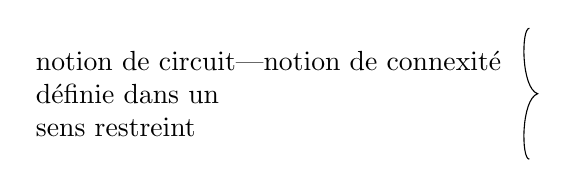
\begin{tikzpicture}
\node[align=left,inner sep=3pt] (m) {\unsure{notion de circuit|notion de connexité}\\\unsure{définie dans un}\\\unsure{sens restreint}};
\draw ([xshift=7pt,yshift=5pt]m.north east)
 .. controls ([xshift=4pt,yshift=5pt]m.north east) and ([xshift=4pt,yshift=2pt]m.east) .. ([xshift=10pt]m.east)
 .. controls ([xshift=4pt,yshift=-2pt]m.east) and ([xshift=4pt,yshift=-5pt]m.south east) .. ([xshift=7pt,yshift=-5pt]m.south east);
\end{tikzpicture}}}
On suppose dorénavant que $\rho$ est \deleted{\unsure{défini}} \inserted{\unsure{prolongé}} sur \unsure{tt} $A$
et que \unsure{$=$} pour l'orientation \unsure{inverse} (ce sont des
propriétés \unsure{combinatoires} de $(A,\sigma,A',\rho)$).
Alors $\rho$ sur $A$ est un \uline{\unsure{autom.}}. Soit $\unsure{\overline S}=A/\rho\supset S$,
$\widehat S\unsure{\subset|=}\overline S$ la partie de $\overline S$ correspondant aux orbites finies.
On peut \unsure{compactifier} \unsure{partiellement} $X$ en \inserted{$\widehat X$}\deleted{\unsure{$\overline X$}}
\unsure{ajoutant} les pts de $\widehat S-S$ (ainsi
que : $\unsure{K^\circ}$\inserted{\unsure{$\simeq\Pi_{0,3}$}}), l'image inverse \inserted{$\widehat A'$} de
$\widehat S$ dans $A$ \inserted{\unsure{contient $A'$ et}}
est \unsure{st.} \unsure{$\forall$} par $\rho$ et $\sigma$
mais \deleted{\unsure{n'est pas|ce n'est pas} néc. égal \unsure{à|avec} $A'$.}
\inserted{: $A$ \unsure{tt entier|est entier}.}

\margin{\figure{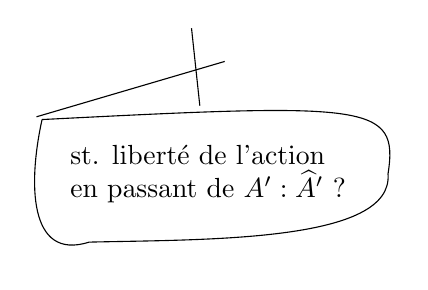
\begin{tikzpicture}
\node[align=left,inner sep=5pt] (m) {\unsure{st. liberté de l'action}\\\unsure{en passant de} $A':\widehat A'$ ?};
\draw ([xshift=-5pt,yshift=4pt]m.north west)
 .. controls ([xshift=-10pt,yshift=-3pt]m.west) and ([xshift=-10pt,yshift=-16pt]m.south west) .. ([xshift=12pt,yshift=-9pt]m.south west)
 .. controls ([yshift=-8pt]m.south) and ([xshift=12pt,yshift=-9pt]m.south east) .. ([xshift=10pt]m.east)
 .. controls ([xshift=14pt,yshift=10pt]m.north east) and ([xshift=3pt,yshift=10pt]m.north east) .. ([xshift=-5pt,yshift=4pt]m.north west);
\draw ([xshift=-7pt,yshift=5pt]m.north west) -- ([xshift=6pt,yshift=25pt]m.north);
\draw ([xshift=-3pt,yshift=9pt]m.north) -- ([xshift=-6pt,yshift=37pt]m.north);
\end{tikzpicture}}}

Les quadruples $(A,\sigma,A',\rho)$ \unsure{satisfaisant} aux
axiomes, \unsure{doivent} \inserted{et tels que $A'=\widehat A'$}
\unsure{s'identifier|s'identifient} aux \deleted{\unsure{triples}} triples
$(A,\sigma,\rho)$ d'un ens. \uline{\unsure{quelc.}} avec un autom.
$\sigma$ d'ordre $2$ \uline{ss pt fixe}, et un autom. $\rho$
\uline{quelc.}. On \unsure{retrouve} $A'$ comme l'ens des
él. de $A$ d'orbite finie sous $\rho$ --- mais on
suppose que $A'\cup\sigma A'=A$.
}

\scanpage{33}
\diagram{\begin{tikzcd}[ampersand replacement=\&,column sep=large,row sep=large]
 0\arrow[r] \& \overset{\omega}{\mathbb Z}\arrow[r,"p"]\arrow[d,"q"'] \& \overset{\widetilde\Pi_0}{\overset{\Vert}{\mathbb Z}}\arrow[r,"\alpha\varphi_p",very thick]\arrow[d] \& \overset{\Pi_0}{\overset{\Vert}{\mathbb Z/p\mathbb Z}}\arrow[r]\arrow[d,equal] \& 0\\
 0\arrow[r,no head,"\overline\omega"'] \& \mathbb Z\arrow[r] \& \widetilde\Pi_0(q)\arrow[r]\arrow[d,"{\substack{\text{\unsure{nul sur }}\widetilde\Pi_0,\\\text{\unsure{can sur }}\mathbb Z\overline\omega}}"] \& \mathbb Z/p\mathbb Z\arrow[r,no head] \& 0\\
 \&\& \mathbb Z/q\mathbb Z \&\&
\end{tikzcd}}
\margin{$\varphi_p:\mathbb Z\longrightarrow\mathbb Z/p\mathbb Z$ hom. can.\\
$\alpha\in(\mathbb Z/p\mathbb Z)^*$\\
\deleted{$\unsure{\beta}\in(\mathbb Z/q\mathbb Z)^*$}}

\diagram{\begin{tikzcd}[ampersand replacement=\&,column sep=large,row sep=large]
 \&\& \overset{\omega}{\mathbb Z}\arrow[r]\arrow[dl,equal] \& \widetilde\Pi_0\arrow[r]\arrow[dl] \& (\mathbb Z/p\mathbb Z\times0)\arrow[dl]\\
 0\arrow[r,no head] \& \overset{\omega}{\mathbb Z}\arrow[r]\arrow[dr,shift right=.6ex] \& \widetilde\Pi_0(q)\arrow[r] \& \mathbb Z/p\mathbb Z\times\mathbb Z/q\mathbb Z\arrow[r,no head] \& 0\\
 \&\& \underset{\omega}{\mathbb Z}\arrow[ul,"q"'{pos=.55},shift right=.6ex]\arrow[r,"\unsure{q}"] \& \underset{\overline\omega}{\mathbb Z}\arrow[ul]\arrow[r,no head] \& 0\times\mathbb Z/q\mathbb Z\arrow[ul]
\end{tikzcd}}
\margin{$\alpha\eta_p$}

\diagram{\begin{tikzcd}[ampersand replacement=\&,column sep=large,row sep=large]
 0\arrow[r,no head] \& \mathbb Z\arrow[r]\arrow[d,equal] \& \widetilde\Pi_0(q)\arrow[r,no head] \& \mathbb Z/p\mathbb Z\times\mathbb Z/q\mathbb Z\arrow[r,no head] \& 0\\
 0\arrow[r,no head] \& \mathbb Z\arrow[r,no head] \& \widetilde\Pi'_0\arrow[r]\arrow[u] \& \mathbb Z/\mu\mathbb Z\arrow[r,no head]\arrow[u,"\delta",very thick] \& 0
\end{tikzcd}}

\deleted{\unsure{L'extension est} \illegible{1} :}
\[
 \unsure{\zeta'|\xi'}\deleted{\unsure{\zeta|\xi}}=
 \mathrm{cl}(\widetilde\Pi'_0)\in
 \operatorname{Ext}^{\unsure{1}}_{\deleted{\unsure{\mathbb Z}}}
 (\mathbb Z/\mu\mathbb Z,\mathbb Z)\simeq\mathbb Z/\mu\mathbb Z
\]
\[
 \deleted{\unsure{=}}\quad
 \unsure{\zeta'|\xi'}=
 \delta^*\!\left(
 \underbrace{\mathrm{cl}(\widetilde\Pi_0\unsure{(q)|q})}_{\unsure{\zeta|\xi}\,\in\,\operatorname{Ext}^1(\mathbb Z/p\mathbb Z\times\mathbb Z/q\mathbb Z,\mathbb Z)}
 \right)\unsure{'}
\]
\[
 \unsure{\zeta|\xi}=
 \mathrm{pr}_1^*\!\left(\underbrace{\mathrm{cl}(\widetilde\Pi_0)}_{\alpha\eta_p}\right)
 +\mathrm{pr}_2^*\!\left(\underbrace{\mathrm{cl}(\mathbb Z)}_{\eta_q}\right)
\]
\[
\begin{array}{ll}
 \delta_p:\mathbb Z/\mu\mathbb Z\mathrel{\overset{\mathrm{can}}{-}}\mathbb Z/p\mathbb Z
 &\unsure{\zeta'|\xi'}=\deleted{q'\eta_\mu+p'\eta_\mu}\\[1ex]
 \delta_q:\mathbb Z/\mu\mathbb Z\mathrel{\overset{\mathrm{can}}{-}}\mathbb Z/q\mathbb Z&\\[1ex]
 \delta_p^*(\eta_p)=q'\eta_\mu & \delta_p^{\unsure{*|' }}(\alpha\eta_p)=q'\alpha\eta_\mu\\[1ex]
 \delta_q^{\unsure{*|'}}(\eta_q)=p'\eta_\mu &
\end{array}
\]
\margin{32}

\scanpage{34}
\deleted{$\unsure{4)}\ \unsure{\widetilde{\mathrm{Sl}}}(2,\mathbb Z)\simeq
\unsure{\mathcal T_{1,1}}\,\unsure{\mathrm{SL}}\,\unsure{\Pi}$}

1)
\[
\begin{gathered}
 S\mathcal T_{11}\simeq\widetilde{\mathrm{Sl}}(2,\mathbb Z)
 \simeq\{\rho,\sigma\mid\underbrace{\rho^3=\sigma^2}_{\omega}\}
 \simeq
 \underset{\substack{\Vert\\\{\rho,\sigma\mid\rho^3=\sigma^2=1\}}}{\Pi_{0,3}^D}
 \times_{\unsure{\mathbb Z/6\mathbb Z}}\mathbb Z\\
 \simeq S\Pi_{0,3}^D
\end{gathered}
\]
\inserted{\deleted{$\unsure{\alpha}$}
\diagram{\begin{tikzcd}[ampersand replacement=\&,row sep=small]
 \rho\arrow[r,mapsto]\&2\\
 \sigma\arrow[r]\&3
\end{tikzcd}}}

% Le bloc suivant est écrit tête-bêche par rapport à la ligne précédente.
\diagram{\begin{tikzcd}[ampersand replacement=\&,column sep=large,row sep=large]
 \widetilde\Pi\arrow[r,no head]\arrow[dd,no head]\&\unsure{\Pi}\arrow[r,no head]\arrow[d]\&\Pi'\arrow[r]\arrow[dd,Rightarrow]\&\Pi\arrow[dd]\\
 \&\mathbb D_3''\arrow[dd]\&\&\\
 \mathbb Z\arrow[rr]\&\&\mathbb Z/12\mathbb Z\arrow[r]\arrow[d]\&\mathbb Z/6\mathbb Z\arrow[d]\\
 \&\unsure{\mathbb Z/}\&\mathbb Z/4\mathbb Z\arrow[r]\&\mathbb Z/2\mathbb Z
\end{tikzcd}}
\margin{$\Pi_0=\mathbb Z/6\mathbb Z$}
\margin{$\Pi_0\times\unsure{7|1}$}
\diagram{\begin{tikzcd}[ampersand replacement=\&,column sep=large,row sep=large]
 \mathbb Z\arrow[r,no head]\&\widetilde\Pi(4)\arrow[r]\&\Pi\times\mathbb Z/4\mathbb Z\arrow[r,no head]\arrow[d]\&1\\
 \&\widetilde\Pi\arrow[u,"?"']\arrow[r,"\uline{\unsure{cart}}"]\&\Pi'\&
\end{tikzcd}}

% Billet préexistant, à lire après une rotation de 90 degrés.
\margin{27-11-81}
M. Grothendieck

A remplir d'urgence

Merci

\uline{R. \unsure{Boucher}}
\margin{33}

\scanpage{35}
\[
 (p'+q'\alpha)\eta_\mu
\]
\[
 p=6,\ q=4\qquad(\alpha=-1\ ?)
\]
\[
 \deleted{\unsure{p}}\ \mu=12\qquad p'=3,\ q'=2
\]
\[
 \deleted{\unsure{p'+}}\ (3-2)\eta_\mu\ !
\]
\figure{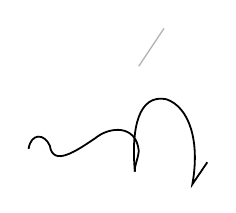
\begin{tikzpicture}[x=1cm,y=1cm]
 \draw[line width=.5pt,opacity=.3] (1.4,1.7)--(1.72,2.18);
 \draw[line width=.65pt] (0,.65) .. controls (.03,.85) and (.2,.85) .. (.27,.69)
 .. controls (.31,.42) and (.6,.62) .. (.84,.78)
 .. controls (1.03,.94) and (1.37,.96) .. (1.4,.62)
 .. controls (1.38,.48) and (1.34,.43) .. (1.35,.36);
 \draw[line width=.65pt] (1.35,.36) .. controls (1.3,.92) and (1.4,1.35) .. (1.75,1.28)
 .. controls (2.04,1.18) and (2.18,.75) .. (2.08,.2)
 --(2.27,.48);
\end{tikzpicture}}

$\cdot$
\diagram{\begin{tikzcd}[ampersand replacement=\&,column sep=large,row sep=small]
 \Pi_{0,3}^D\arrow[r,"{-\alpha}"{draw,circle,inner sep=1pt},very thick]\&\mathbb Z/6\mathbb Z\\
 \rho\arrow[r,mapsto]\&-2\ \mathrm{mod}\ 6\\
 \sigma\arrow[r,mapsto]\&3\ \mathrm{mod}\ 6\\[1ex]
 \varepsilon_0=\sigma\rho\arrow[r,mapsto,very thick]\&1\ \mathrm{mod}\ 6\\
 \rho_0=\varepsilon_0^2\arrow[r,mapsto]\&2\ \mathrm{mod}\ 6
\end{tikzcd}}
\deleted{$\unsure{\varphi}$}
% Marques très pâles à droite des résidus; possible transparence du verso.
\margin{$\unsure{\Gamma|\sqrt{\phantom{x}}}$\\$\unsure{\xi_0\prime|\xi_0}$\\$\unsure{t\prime r|t\prime h}$}

\margin{défini directement par l'action de $\Pi_{0,3}^D$ sur le
\unsure{revêt}\deleted{\unsure{ement}} principal de $(U_{0,3},\mathfrak S_3)$
de groupe $\mathbb Z/6\mathbb Z$, défini par
la \unsure{multisection|multiplication} \inserted{canonique} de
\deleted{$\unsure{\mathcal O(1)}$}$\mathcal O_{U_{0,3}}(1)^*$
$=PU_{0,3}$}

\[
 \widetilde\Pi_{0,3}^D
\]
\deleted{$\mathcal O\unsure{(1)}$}
\diagram{\begin{tikzcd}[ampersand replacement=\&,column sep=small,row sep=large]
 U'_{0,3}\arrow[rr,phantom,"\subset"]\arrow[dr,no head,"{\mu_6\text{-}\unsure{\mathrm{rev}^{\mathrm t}}}"']\&\&PU_{0,3}\arrow[dl,no head]\&\unsure{+}\\
 \&U_{0,3}\&\&
\end{tikzcd}}
\deleted{$\unsure{\longrightarrow}$}

\diagram{\begin{tikzcd}[ampersand replacement=\&,column sep=large,row sep=large]
 \&\Pi_{0,3}^D\arrow[r,"{\alpha'}"{draw,circle,inner sep=1pt},very thick]\&\mathbb Z/6\mathbb Z\\
 \pi_1(PU_{0,3},\mathfrak S_3)\arrow[r,equal]\&\widetilde\Pi_{0,3}^D\arrow[u]\arrow[r]\&\mathbb Z\arrow[u]\\
 \&\omega'\in\mathbb Z\arrow[u]\arrow[r,"\unsure{=}"]\&\mathbb Z\arrow[u,"6"]
\end{tikzcd}}

\diagram{\begin{tikzcd}[ampersand replacement=\&,column sep=large,row sep=large]
 1\arrow[r]\&\mathbb Z\arrow[r]\arrow[d,equal]\&
 \underset{\substack{\Vert\\\pi_1(PU_{0,3},\mathfrak S_3\times\mu_4)}}{\widetilde\Pi_{0,3}^D(4)}\arrow[r,very thick]\&
 \Pi_{0,3}^D\times\mathbb Z/4\mathbb Z\arrow[r]\&1\\
 1\arrow[r,no head]\&\mathbb Z\arrow[r]\&\widetilde{\mathcal T}_{11}\arrow[u,bend left=20]\arrow[r,Rightarrow]\&
 \mathcal T_{1,1}=\Pi_{0,3}^D\times_{\mathbb Z/2\mathbb Z}\mathbb Z/4\mathbb Z\arrow[u,hook]\&
\end{tikzcd}}

\deleted{$\unsure{\widetilde\Pi_{0,3}^D}\,\unsure{\mathbb Z/4\mathbb Z}\longrightarrow$}
\[
\begin{array}{ll}
 \widetilde\Pi_{0,3}^D\ni\widetilde\rho^{\unsure{\sharp|'}}=(\rho,-2)
 &\widetilde\rho^{\unsure{\sharp}3}=\widetilde\sigma^{\unsure{\sharp}2}=\omega'\\
 \hfill\widetilde\sigma^{\unsure{\sharp|'}}=(\sigma,-3)&
\end{array}
\]
\diagram{\begin{tikzcd}[ampersand replacement=\&,column sep=small,row sep=small]
 \widetilde\rho,\arrow[d]\&\widetilde\sigma\arrow[d]\&
 \in\widetilde\Pi_{0,3}^D=
 \left\{\widetilde\rho,\widetilde\sigma\mid
 \underbrace{\widetilde\rho^3=\widetilde\sigma^2}_{\unsure{\omega'^{-1}|\widetilde\omega^{-1}}=\unsure{\omega|\infty}}
 \deleted{\unsure{\omega\in\mathbb Z}}\right\}\\
 \rho\&\sigma\&\simeq\widetilde{\mathcal T}_{11}
\end{tikzcd}}
\margin{34}

\scanpage{36}
\diagram{\begin{tikzcd}[ampersand replacement=\&,column sep=large,row sep=large,column sep=9pt,row sep=14pt,execute at begin picture={\fontsize{10}{12}\selectfont}]
 \&\&\left\{\rho,\sigma\mid\underbrace{\rho^3=\sigma^2}_{\omega'^{-1}=\omega}\right\}\deleted{\unsure{\omega|\infty}}\arrow[d,equal]\&\&\\
 1\arrow[r,no head]\&\overset{\omega'=\unsure{\omega^{-1}|\overline\omega'}}{\mathbb Z}\arrow[r]\arrow[d,equal]\&S\Pi_{0,3}^D\arrow[r]\arrow[d]\&\Pi_{0,3}^D\arrow[r,no head]\arrow[d]\&1\\
 1\arrow[r,no head]\&\mathbb Z\arrow[r]\&S\Pi_{0,3}^D(4)\arrow[r]\&\Pi_{0,3}^D\times\mathbb Z/4\mathbb Z\arrow[r,no head]\&1\\[4em]
 1\arrow[r]\&\underset{\omega^2}{\mathbb Z}\arrow[r]\arrow[u,very thick]\&S\mathcal T_{11}\arrow[r]\arrow[u,very thick,"{\underbrace{\begin{gathered}\rho\mapsto\rho\overline\omega^2\\\sigma\mapsto\sigma\overline\omega^3\\\omega\longrightarrow\overline\omega^2\\\omega^2\longrightarrow\overline\omega^4=\omega'\end{gathered}}}"]\&\mathcal T_{11}\arrow[u,hook,"{\substack{\rho\mapsto(\rho,2)\\\sigma\mapsto(\sigma,3)}}"]\&\omega\longrightarrow(1,2)
\end{tikzcd}}
\margin{$S\Pi_{0,3}^D(4)=\left\{\rho,\sigma,\overline\omega\mid\begin{gathered}\rho^3=\sigma^2=\overline\omega^{-4}\\\overline\omega\ \text{central}\end{gathered}\right\}$\\
NB $\unsure{\dot{\overline\omega}|\overline\omega}^{4}=\unsure{\omega^{-1}}$\\
$=\omega'\deleted{\unsure{\omega}}$}

% Groupe et flèche au pied du feuillet, écrits tête-bêche.
\diagram{\begin{tikzcd}[ampersand replacement=\&,column sep=large]
 \overbrace{S\Pi_{0,3}^D(4)}^{\pi_1(U_{0,3},\mathfrak S_3\times\mu_4)}\arrow[r]\&\Pi_{0,3}^D
\end{tikzcd}}
\margin{35}

\scanpage{37}
% not manuscript: formulaire vierge « ANNEXE II », renseignements à fournir par le candidat devant soutenir une thèse de doctorat d'État, Université des Sciences et Techniques du Languedoc, imprimé tête-bêche.
\margin{36}
